%% ============================================================
%% HallucinationGuard — Paper 1
%% A Taxonomy and Multi-Metric Benchmark of Hallucination
%% in Instruction-Tuned Large Language Models
%%
%% Author: Monishwaran K
%% Institution: Sathyabama Institute of Science and Technology
%% ============================================================

\documentclass[conference]{IEEEtran}

%% --- Packages ---
\usepackage{cite}
\usepackage{amsmath,amssymb,amsfonts}
\usepackage{algorithmic}
\usepackage{graphicx}
\usepackage{textcomp}
\usepackage{xcolor}
\usepackage{booktabs}
\usepackage{multirow}
\usepackage{url}
\usepackage{hyperref}
\usepackage{array}
\usepackage{tabularx}

\graphicspath{{figures/}}

%% ============================================================
\begin{document}

\title{A Taxonomy and Multi-Metric Benchmark of Hallucination
in Instruction-Tuned Large Language Models}

\author{
\IEEEauthorblockN{Monishwaran K}
\IEEEauthorblockA{
  \textit{Department of Computer Science and Engineering}\\
  \textit{Sathyabama Institute of Science and Technology}\\
  Chennai, India\\
  monishwarank06@gmail.com
}
}

\maketitle

%% ============================================================
\begin{abstract}
Hallucination in large language models (LLMs) — the generation
of plausible yet factually incorrect content — poses a critical
threat to the reliable deployment of AI systems in high-stakes
domains including healthcare, law, and finance.
Despite growing interest in this problem, a systematic
characterisation of hallucination behaviour across knowledge
domains, together with a rigorous comparison of detection
metrics, remains lacking for instruction-tuned models at the
sub-1B parameter scale.
In this paper, we present a comprehensive taxonomy and
multi-metric benchmark of hallucination in
\textit{google/flan-t5-base}, an instruction-tuned
sequence-to-sequence model, evaluated on the TruthfulQA
dataset comprising 817 questions across 38 knowledge categories.
We evaluate hallucination using three complementary detection
methods — string matching, BERTScore semantic similarity, and
Natural Language Inference (NLI) entailment scoring — and
introduce a consensus-based labelling scheme to resolve
inter-metric disagreement, which we observe in 47.4\% of cases.
Our experiments reveal a consensus hallucination rate of 91.7\%,
with 16 of 38 categories exhibiting complete hallucination
(100\% rate), including History, Politics, Finance, and
Misquotations.
High-stakes domains such as Health (89.1\%) and Law (87.5\%)
demonstrate consistently elevated hallucination rates.
We release our annotated dataset, scoring pipeline, and
experimental code as an open-source benchmark to support
reproducible hallucination research.
\end{abstract}

\begin{IEEEkeywords}
large language models, hallucination detection, natural language
inference, BERTScore, TruthfulQA, benchmark, instruction tuning,
factuality evaluation
\end{IEEEkeywords}

%% ============================================================
\section{Introduction}
\label{sec:introduction}

The widespread deployment of large language models (LLMs) in
production systems has brought renewed urgency to the problem
of \textit{hallucination} — a phenomenon in which generative
models produce fluent, confident, and contextually plausible
responses that are nonetheless factually incorrect
\cite{huang2023survey}.
Hallucination poses particular risks in safety-critical
applications: a medical assistant that fabricates drug
interactions, a legal research tool that invents case citations,
or a financial advisor that generates false market statistics
can cause direct, measurable harm to end users
\cite{ji2023survey}.

Industry estimates suggest that hallucination-related incidents
cost enterprise AI deployments in excess of \$250 million
annually \cite{guardrails2024}.
Despite this, the research community lacks a systematic,
domain-stratified characterisation of hallucination behaviour
for smaller instruction-tuned models that are commonly deployed
in resource-constrained production environments.

Prior work has addressed hallucination detection through a
variety of methods including external knowledge retrieval
\cite{varshney2023stitch}, consistency-based sampling
\cite{manakul2023selfcheck}, and fine-grained atomic evaluation
\cite{min2023factscore}.
However, these studies predominantly evaluate large proprietary
models (GPT-3, GPT-4, ChatGPT) and do not systematically
characterise which knowledge domains are most susceptible to
hallucination, nor do they compare multiple detection metrics
on the same experimental corpus.

This paper addresses these gaps through four contributions:

\begin{enumerate}
\item We present a \textbf{domain-stratified hallucination
  taxonomy} across 38 knowledge categories using TruthfulQA,
  identifying 16 categories with 100\% hallucination rates.

\item We conduct a \textbf{systematic comparison of three
  detection metrics} — string matching, BERTScore, and NLI
  entailment scoring — on an identical experimental corpus,
  revealing substantial inter-metric disagreement in 47.4\%
  of cases.

\item We propose a \textbf{consensus-based labelling scheme}
  that resolves inter-metric disagreement and provides more
  reliable hallucination labels than any single metric alone.

\item We release an \textbf{open-source benchmark pipeline}
  and annotated dataset to enable reproducible hallucination
  research on instruction-tuned models.
\end{enumerate}

The remainder of this paper is structured as follows.
Section~\ref{sec:related} reviews related work.
Section~\ref{sec:methodology} describes our experimental
methodology.
Section~\ref{sec:results} presents quantitative results.
Section~\ref{sec:discussion} analyses key findings.
Section~\ref{sec:conclusion} concludes and outlines future work.

%% ============================================================
\section{Related Work}
\label{sec:related}

\subsection{Hallucination in Language Models}

Hallucination in natural language generation systems was first
systematically studied by Ji et al.~\cite{ji2023survey}, who
provided an early taxonomy distinguishing intrinsic
hallucinations (contradicting source material) from extrinsic
hallucinations (introducing unverifiable information).
Huang et al.~\cite{huang2023survey} extended this taxonomy in
the context of LLMs, categorising hallucinations into factuality
errors, faithfulness errors, reasoning errors, and
instruction-following failures, and reviewed detection and
mitigation strategies across each type.

Lin et al.~\cite{lin2022truthfulqa} introduced TruthfulQA, a
benchmark of 817 adversarially constructed questions targeting
common human misconceptions, demonstrating that larger LLMs
are not necessarily more truthful.
Their study showed that GPT-3 achieved truthfulness on only
58\% of questions, motivating further research into both
detection and mitigation.

\subsection{Hallucination Detection Methods}

Manakul et al.~\cite{manakul2023selfcheck} proposed
SelfCheckGPT, a zero-resource black-box detection approach
that samples multiple responses from a model and measures
information consistency using BERTScore, NLI, and n-gram
overlap.
Their key insight — that hallucinated facts produce
inconsistent samples while factual claims produce consistent
ones — directly motivates our multi-metric evaluation
framework.

Min et al.~\cite{min2023factscore} introduced FActScore,
a fine-grained evaluation metric that decomposes generated
text into atomic facts and verifies each against a knowledge
source, achieving less than 2\% error compared to human
annotation.

Varshney et al.~\cite{varshney2023stitch} demonstrated that
early detection of likely-to-hallucinate tokens allows
targeted intervention, reducing hallucination without
full regeneration.

\subsection{Gaps Addressed by This Work}

Existing benchmarks predominantly target large proprietary
models and do not provide domain-stratified analysis across
knowledge categories.
Furthermore, no study has systematically compared string
matching, BERTScore, and NLI entailment on the same corpus
to quantify inter-metric disagreement.
This paper addresses both gaps directly.

%% ============================================================
\section{Methodology}
\label{sec:methodology}

\subsection{Dataset}

We evaluate on TruthfulQA \cite{lin2022truthfulqa} in its
generation configuration, comprising 817 questions across
38 knowledge categories.
Table~\ref{tab:dataset_stats} summarises dataset statistics.
Categories span misconceptions, law, health, sociology,
history, conspiracies, and 32 additional domains, with
Misconceptions being the largest category (n=100, 12.24\%).
Each question includes one best answer, a list of acceptable
correct answers (mean: 3.18 per question), and a list of
known incorrect answers that plausible-but-wrong models
tend to produce (mean: 4.06 per question).

\begin{table}[h]
\caption{TruthfulQA Dataset Statistics}
\label{tab:dataset_stats}
\centering
\begin{tabular}{lc}
\toprule
\textbf{Metric} & \textbf{Value} \\
\midrule
Total questions & 817 \\
Unique categories & 38 \\
Largest category (Misconceptions) & 100 (12.24\%) \\
Mean answer length (words) & 9.22 \\
Std. dev. answer length & 4.08 \\
Mean correct answers per question & 3.18 \\
Mean incorrect answers per question & 4.06 \\
\bottomrule
\end{tabular}
\end{table}

\subsection{Model}

We evaluate \textit{google/flan-t5-base}
\cite{chung2022scaling}, an instruction-tuned
sequence-to-sequence model with approximately 250M parameters.
Flan-T5-Base represents a class of compact, openly available
instruction-tuned models that are widely deployed in
resource-constrained environments.
The model was queried using beam search with 4 beams and a
maximum generation length of 100 tokens.
All experiments were conducted on a single NVIDIA T4 GPU
(16GB VRAM) via Google Colaboratory.

\subsection{Detection Methods}

We evaluate three complementary hallucination detection
methods, each operating on the pair
($r$, $A^+$) where $r$ is the model response and
$A^+$ is the set of correct reference answers.

\subsubsection{String Matching (Baseline)}
We compute exact match (EM) and partial match (PM) between
the model response and the reference answer set.
A response is labelled \textit{correct} if it exactly matches
or is contained within any reference answer, and
\textit{hallucinated} otherwise.
This serves as a fast, interpretable baseline.

\subsubsection{BERTScore}
BERTScore \cite{zhang2020bertscore} computes token-level
cosine similarity between BERT embeddings of the candidate
and reference texts, aggregated as precision, recall,
and F1.
We use \textit{bert-base-uncased} and apply a threshold
of F1~$\geq$~0.85 to classify responses as correct,
following the calibration recommended in the original paper.

\subsubsection{NLI Entailment Score}
We employ \textit{facebook/bart-large-mnli} as a
zero-shot natural language inference classifier.
For each response pair $(r, a^*)$ where $a^*$ is the
best reference answer, we compute the entailment probability
$P(\text{entail} \mid r, a^*)$.
Responses with entailment probability $>$~0.5 are
classified as correct; all others as hallucinated.
This method captures logical consistency beyond surface-level
lexical overlap.

\subsubsection{Consensus Labelling}
Given three binary labels $\{l_1, l_2, l_3\}$ from the
above methods, we assign a consensus label of
\textit{hallucinated} when at least two of three methods
agree on hallucination, and \textit{correct} otherwise.
This majority-vote scheme reduces the impact of
individual metric bias and provides more stable labels
for downstream analysis.

%% ============================================================
\section{Results}
\label{sec:results}

\subsection{Overall Hallucination Rates}

Table~\ref{tab:method_comparison} presents the hallucination
rates computed by each detection method.
The consensus method yields a hallucination rate of 91.7\%
(749 of 817 responses), reflecting that
\textit{google/flan-t5-base} fails to produce truthful
responses on the large majority of TruthfulQA questions.

\begin{table}[h]
\caption{Hallucination Rates by Detection Method}
\label{tab:method_comparison}
\centering
\begin{tabular}{lccc}
\toprule
\textbf{Method} & \textbf{Correct} &
\textbf{Hallucinated} & \textbf{Rate (\%)} \\
\midrule
String Match (Baseline) & 123 & 694 & 84.9 \\
BERTScore (F1 $\geq$ 0.85) & 3 & 814 & 99.6 \\
NLI Entailment & 331 & 486 & 59.5 \\
\textbf{Consensus ($\geq$2 methods)} & \textbf{68} &
\textbf{749} & \textbf{91.7} \\
\bottomrule
\end{tabular}
\end{table}

Fig.~\ref{fig:metric_comparison} illustrates the
substantial variation in reported hallucination rates
across methods, ranging from 59.5\% (NLI) to 99.6\%
(BERTScore).
This 40.1 percentage-point spread motivates the use of
a consensus approach rather than reliance on any single
metric.

\begin{figure}[h]
\centering

\includegraphics[width=\columnwidth]
  {fig03_metric_comparison.png}
\caption{Hallucination rates across three detection methods
and the consensus scheme. The 40.1pp spread demonstrates
that metric choice substantially affects reported results.}
\label{fig:metric_comparison}
\end{figure}

\subsection{Inter-Metric Disagreement}

We observe that 47.4\% of responses (387 of 817) receive
different labels from at least one method, indicating
substantial inter-metric disagreement.
Only 52.5\% of responses are unanimously labelled as
hallucinated, and a mere 0.1\% are unanimously labelled
as correct.
This finding directly motivates the consensus labelling
scheme introduced in Section~\ref{sec:methodology}.

\subsection{BERTScore Distribution}

Fig.~\ref{fig:bertscore_dist} shows the distribution of
BERTScore F1 values across all 817 responses.
The distribution is centred at a mean F1 of 0.387
(std. dev. 0.101), with 74.1\% of responses falling
in the 0.3--0.5 range.
This distribution is characteristic of responses that
exhibit surface-level word overlap with correct answers
but are semantically divergent — a defining property
of factuality hallucination as opposed to random
noise generation.

\begin{figure}[h]
\centering
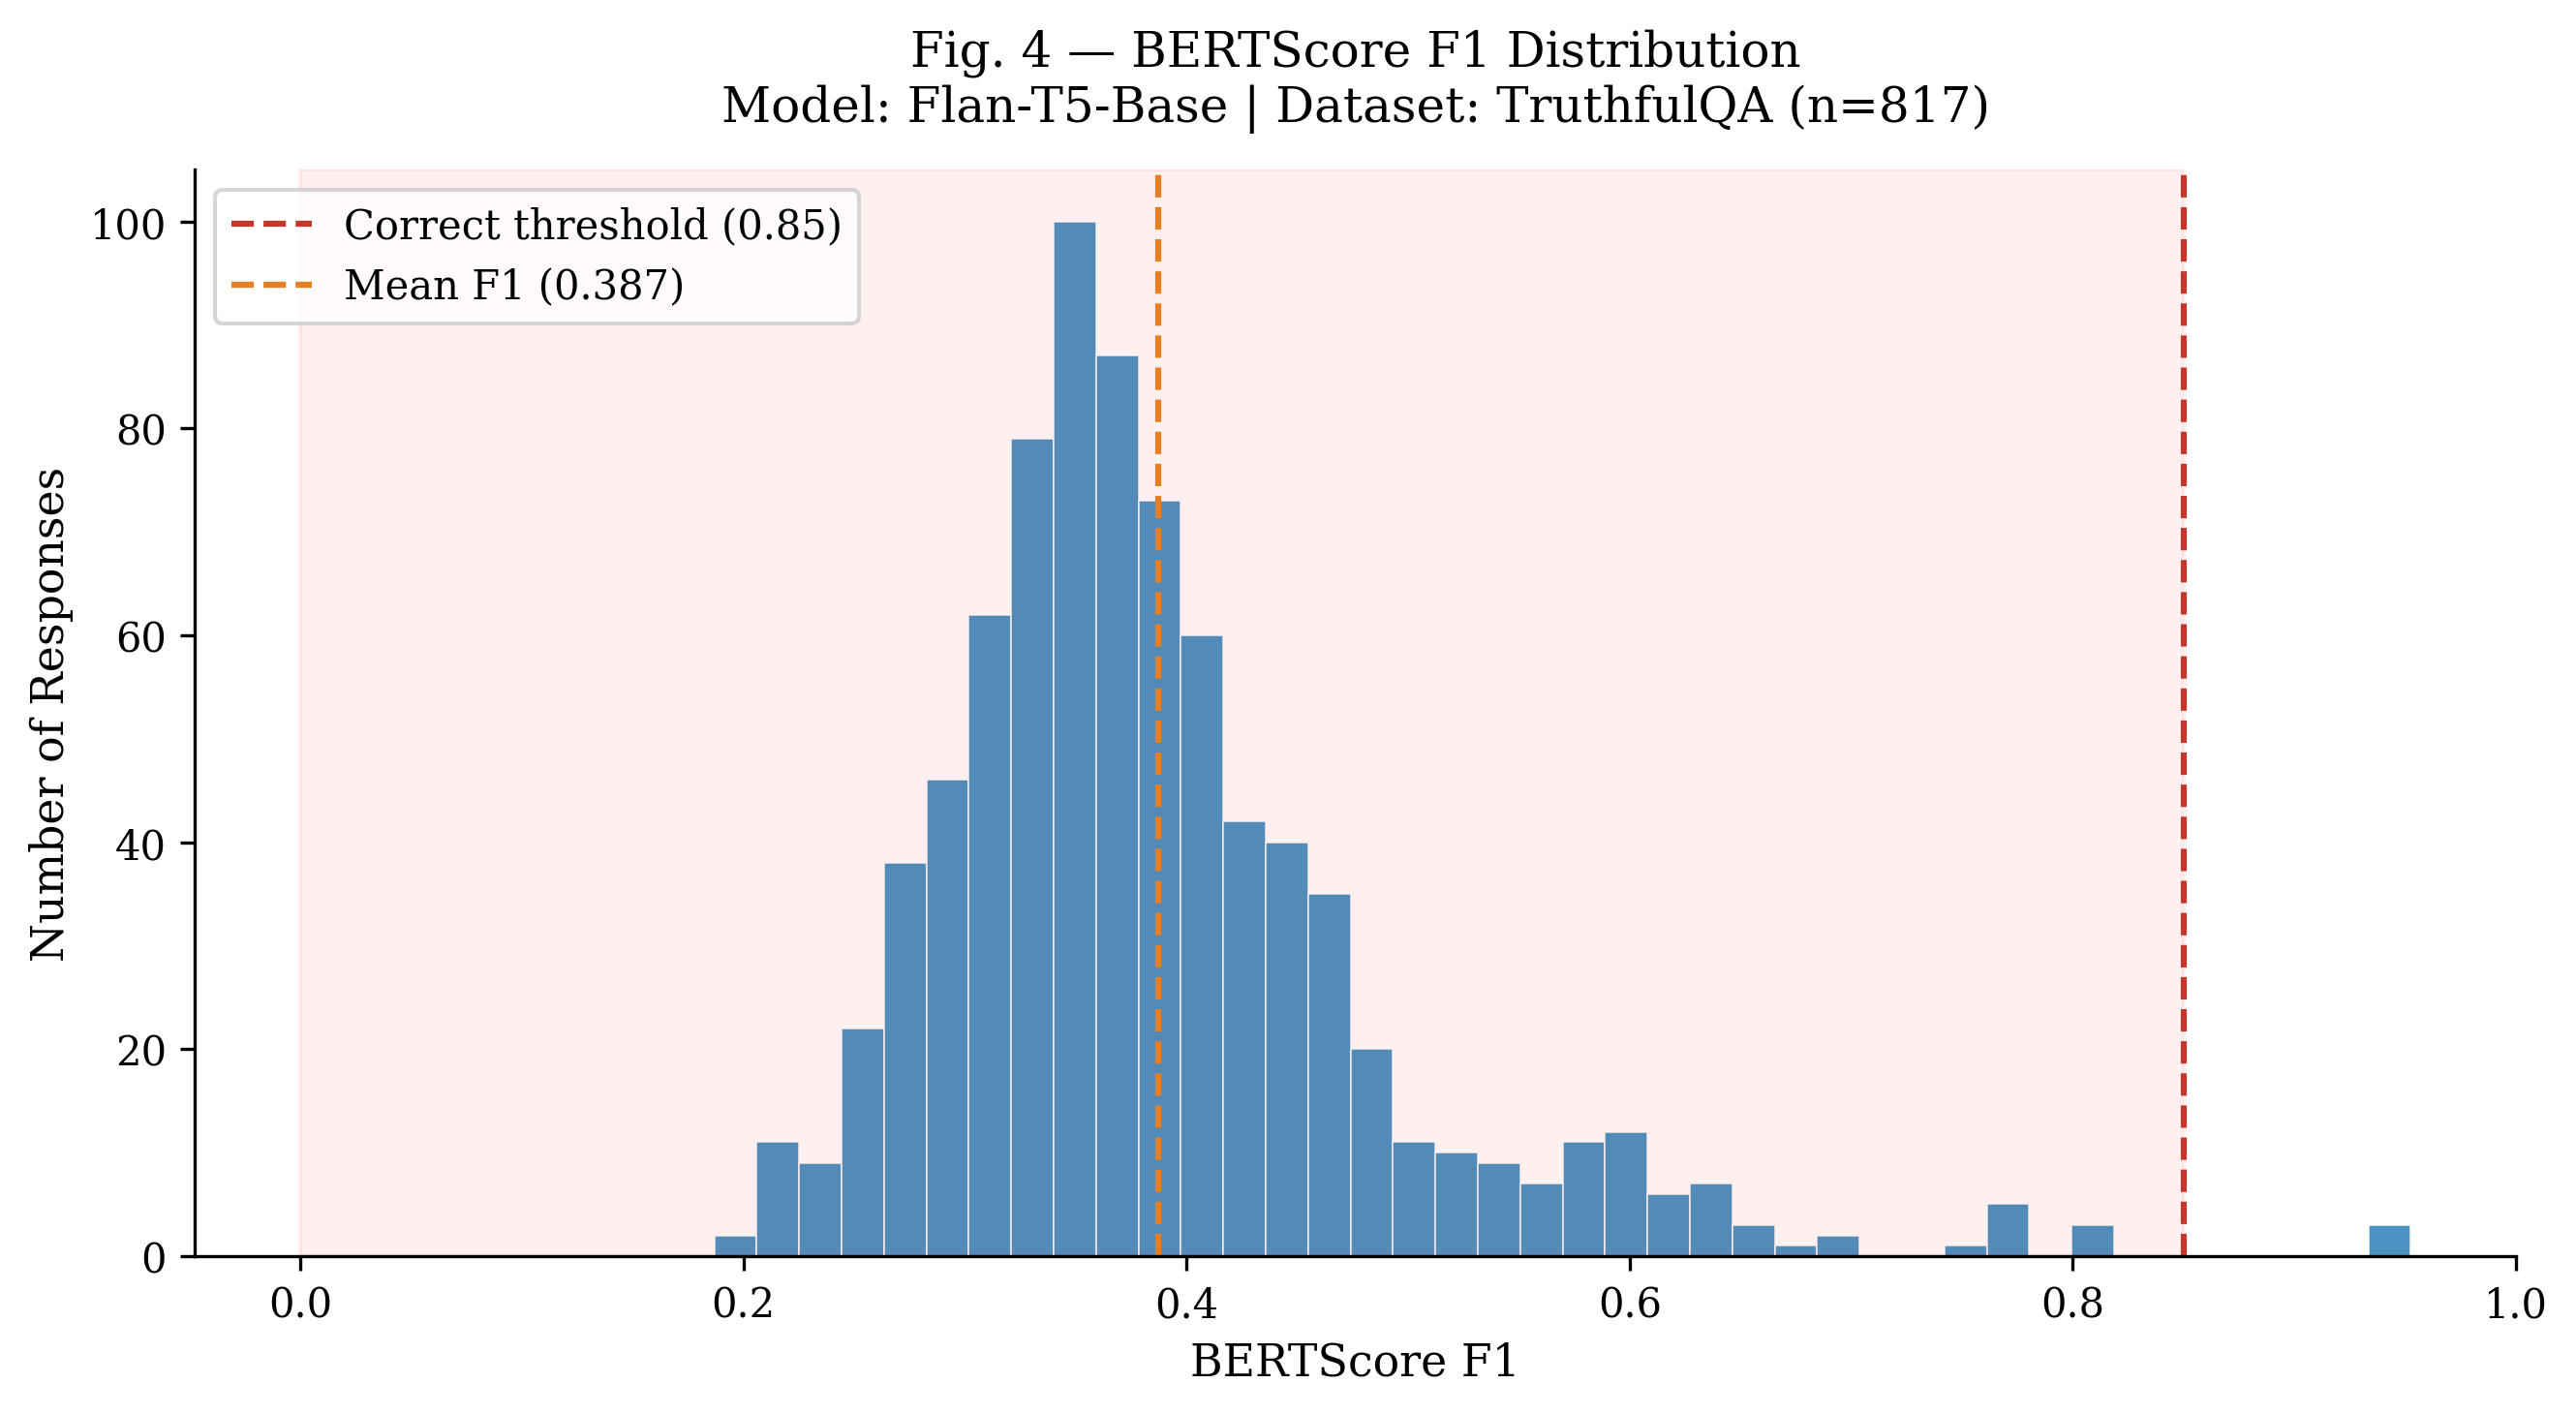
\includegraphics[width=\columnwidth]
  {fig04_bertscore_distribution.png}
\caption{BERTScore F1 distribution showing the majority
of responses clustering below the correctness threshold
of 0.85, with a mean of 0.387.}
\label{fig:bertscore_dist}
\end{figure}

\subsection{Domain-Stratified Hallucination Taxonomy}

Fig.~\ref{fig:category_rates} presents consensus
hallucination rates across all 38 TruthfulQA categories.
We identify four tiers of hallucination risk:

\begin{itemize}
\item \textbf{Critical (100\%):} 16 categories including
  History, Politics, Finance, Misquotations, Conspiracies,
  Superstitions, and Paranormal exhibit complete
  hallucination — no correct responses were generated.

\item \textbf{High (85--99\%):} 16 categories including
  Fiction (96.7\%), Misconceptions (93.0\%), Health (89.1\%),
  and Law (87.5\%) demonstrate persistently elevated
  hallucination rates.

\item \textbf{Medium (70--84\%):} 4 categories including
  Nutrition (81.2\%) and Economics (80.6\%).

\item \textbf{Lower ($<$70\%):} 2 categories —
  Proverbs (66.7\%) and Misconceptions: Topical (50.0\%) —
  show relatively lower but still substantial
  hallucination rates.
\end{itemize}

\begin{figure}[h]
\centering
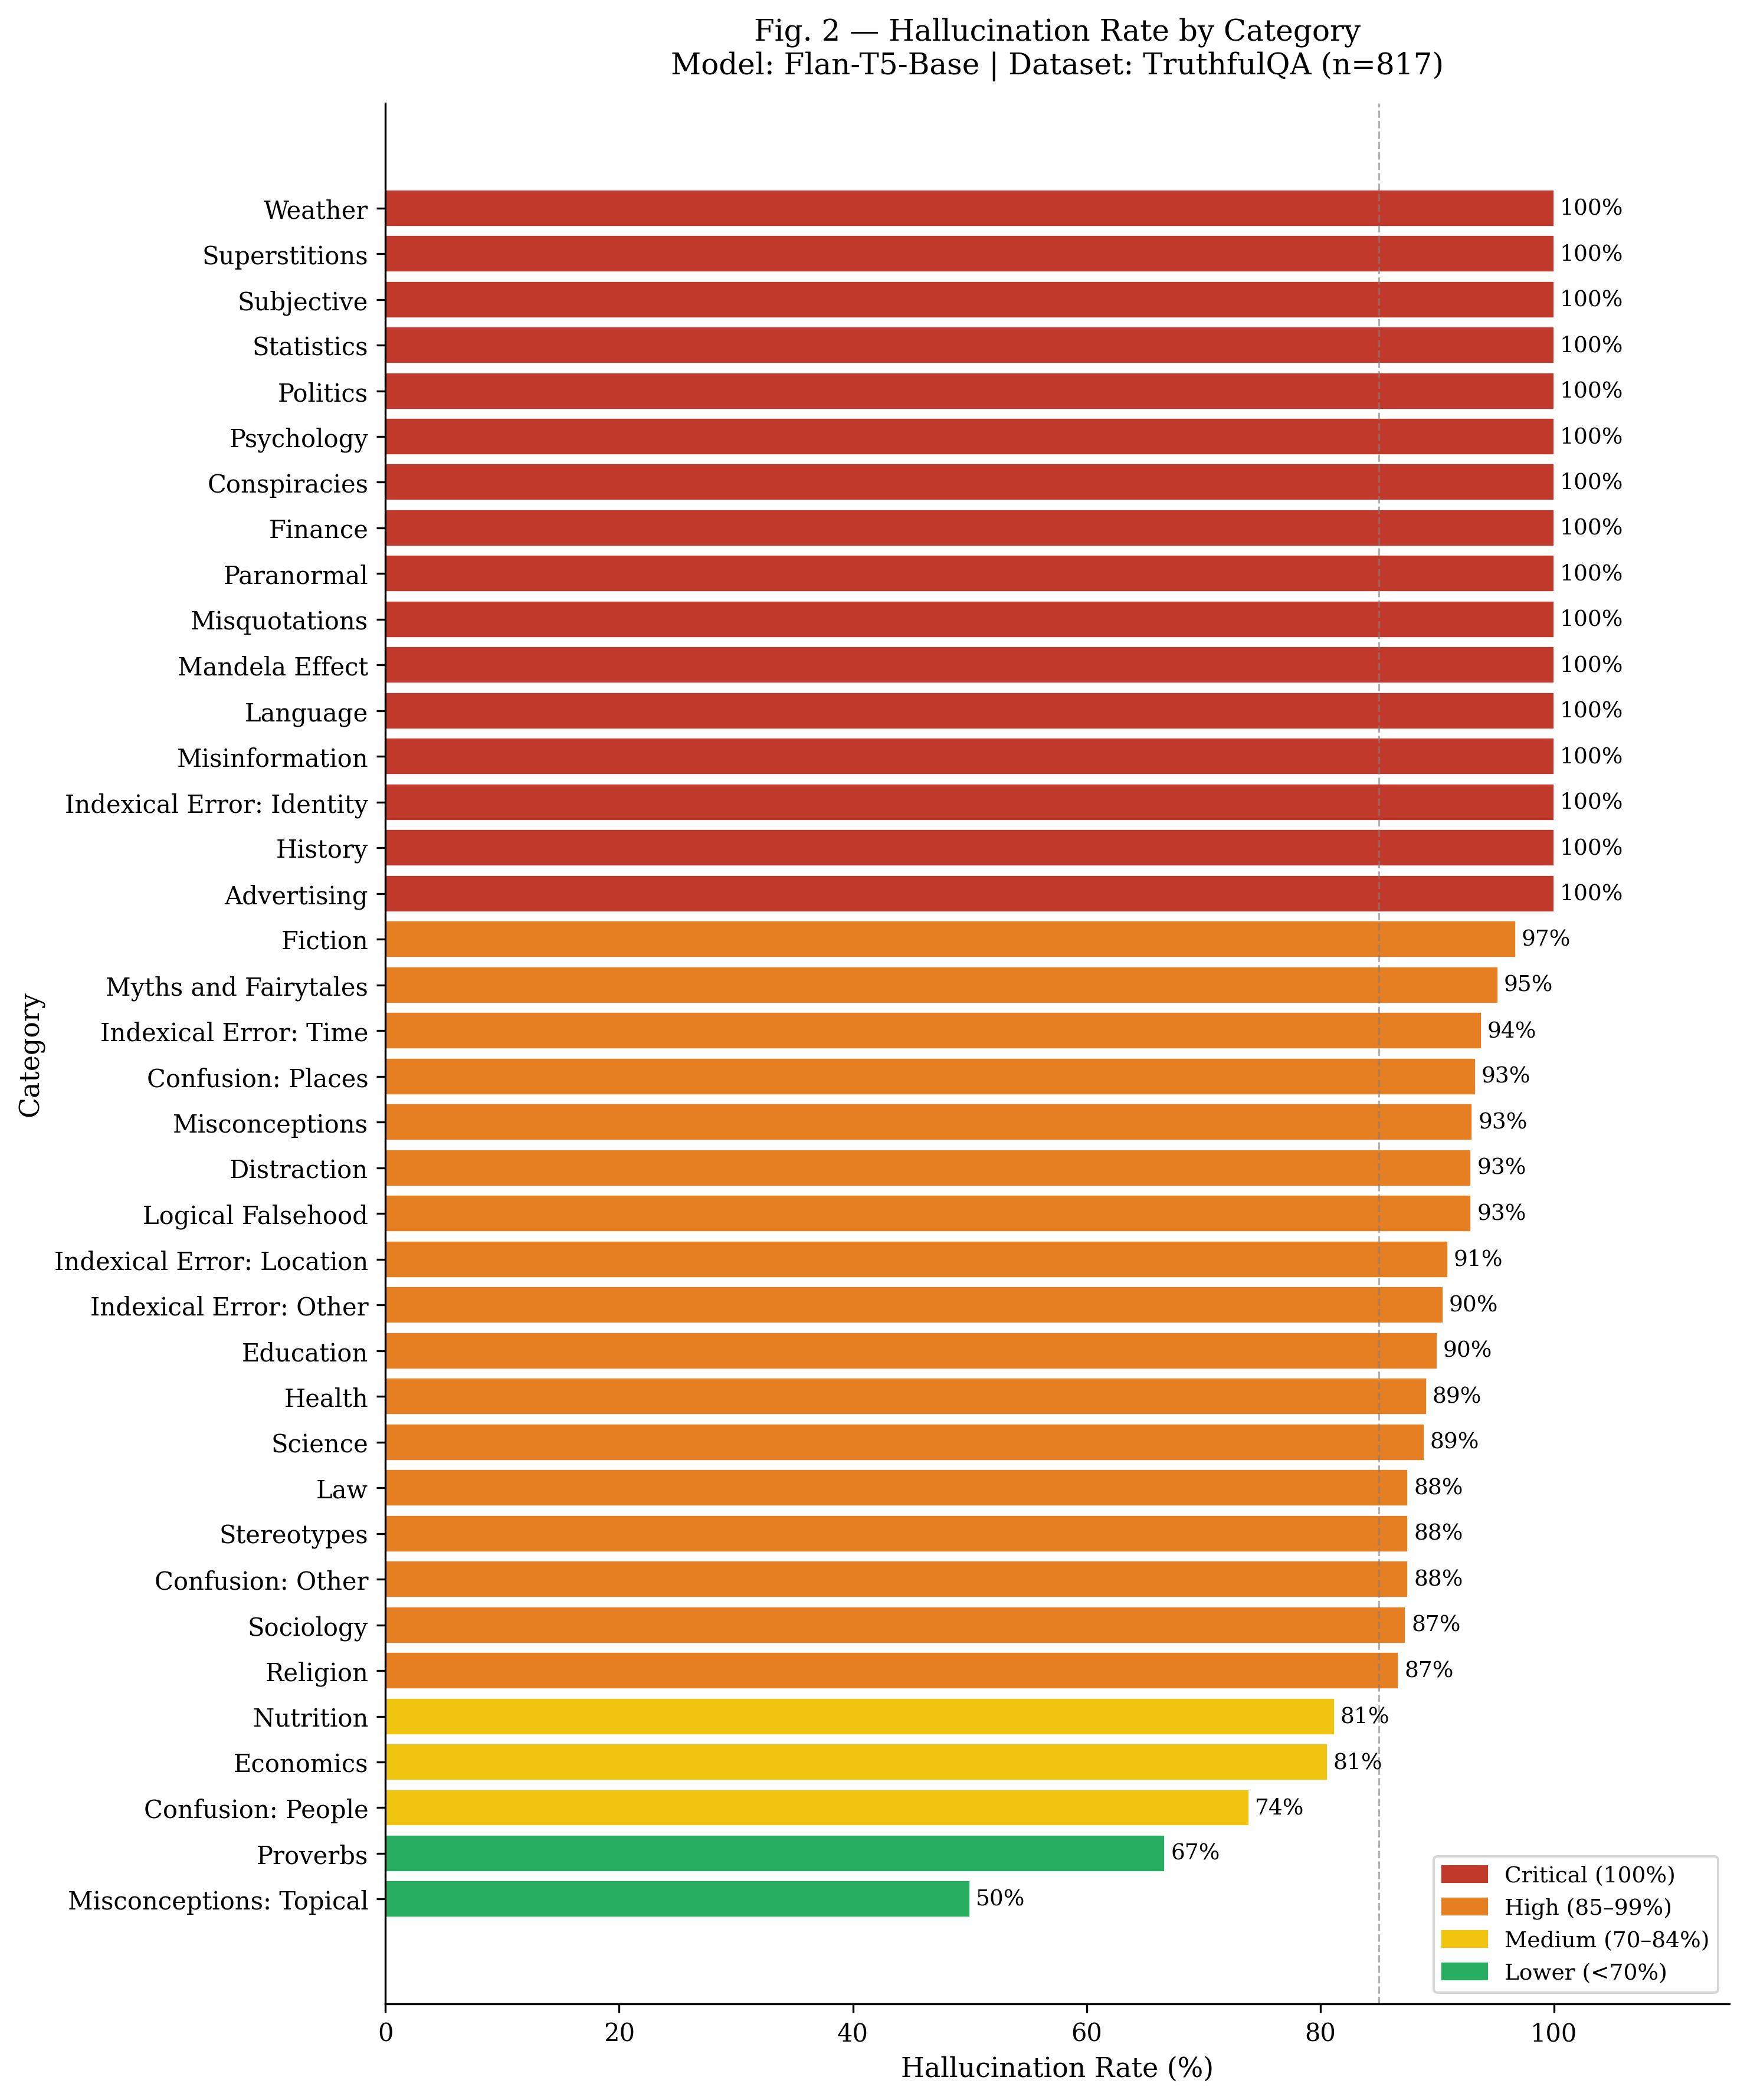
\includegraphics[width=\columnwidth]
  {fig02_hallucination_rate_by_category.png}
\caption{Consensus hallucination rate across all 38
TruthfulQA categories. 16 categories exhibit 100\%
hallucination. High-stakes domains Health and Law
reach 89.1\% and 87.5\% respectively.}
\label{fig:category_rates}
\end{figure}

%% ============================================================
\section{Discussion}
\label{sec:discussion}

\subsection{Metric Disagreement as a Research Signal}

The 47.4\% inter-metric disagreement rate is not a
methodological weakness — it is a finding.
It demonstrates that hallucination is not a binary,
easily-detected property but rather a continuous,
multi-dimensional phenomenon that different measurement
frameworks capture differently.
BERTScore is highly sensitive to semantic divergence,
producing the highest hallucination rate (99.6\%),
while NLI entailment is more lenient, tolerating responses
that do not logically contradict the reference (59.5\%).
String matching occupies an intermediate position (84.9\%).

This result has a direct practical implication:
researchers who report hallucination rates without
specifying their detection methodology are not reporting
comparable results.
Our consensus framework provides a more stable and
reproducible measurement standard.

\subsection{Domain Risk Hierarchy}

The identification of 16 categories with 100\% hallucination
rates reveals a systematic pattern: domains requiring
precise recall of specific cultural, historical, or
factual details (Misquotations, Mandela Effect, History)
are completely beyond the factual reach of Flan-T5-Base.

More critically, high-stakes domains — Health (89.1\%)
and Law (87.5\%) — exhibit hallucination rates that
render unmitigated deployment of this model class
inadvisable in clinical or legal contexts.
This finding motivates targeted mitigation research
for domain-specific LLM deployment, which we address
in subsequent work through a RAG-based mitigation
framework.

\subsection{Implications for Model Scale}

The results presented in this study reflect the behaviour of
a compact 250M parameter model, and it is reasonable to ask
whether larger models would exhibit meaningfully lower
hallucination rates on the same benchmark.
Based on the scaling literature \cite{huang2023survey} and
the findings of Lin et al.~\cite{lin2022truthfulqa}, larger
models do demonstrate improved truthfulness — however, they
do not eliminate hallucination.
Rather, the nature of the failure changes: larger models
tend to hallucinate less frequently, but when they do, their
responses are more linguistically fluent and therefore
more difficult to detect.
A 7B parameter model producing a confident, well-structured
incorrect answer is arguably more dangerous in a high-stakes
deployment than a 250M parameter model producing a short,
obviously incomplete one.
This distinction motivates our subsequent work on
detection and mitigation, where we specifically target
the harder problem of hallucination in larger, more
capable models.

\subsection{Limitations}

This study evaluates a single model (Flan-T5-Base) on a
single benchmark (TruthfulQA).
While TruthfulQA provides broad domain coverage, it was
constructed to maximise difficulty and may not be
representative of real-world query distributions.
The BERTScore threshold of 0.85 was adopted from the
original paper calibration and may require adjustment
for specific domains.
Future work will extend this benchmark to include
Mistral-7B, LLaMA-3-8B, and domain-specific datasets
in medical and legal question answering.

%% ============================================================
\section{Conclusion}
\label{sec:conclusion}

This paper presented a systematic taxonomy and multi-metric
benchmark of hallucination in \textit{google/flan-t5-base}
evaluated on TruthfulQA.
Our key findings are: (1) a consensus hallucination rate
of 91.7\% demonstrating that compact instruction-tuned
models remain highly unreliable on factual question
answering; (2) 16 of 38 knowledge categories exhibit
100\% hallucination rates, including high-stakes domains
of Health and Law; and (3) inter-metric disagreement
in 47.4\% of cases motivates consensus-based evaluation
as a more reliable measurement standard than any single
metric.

We release the complete experimental pipeline, annotated
dataset, and figures as open-source contributions at:
\texttt{https://github.com/monish1402/hallucination-guard}

Future work will extend this benchmark to larger open-source
models, introduce cross-lingual evaluation, and integrate
the scoring pipeline with the detection and mitigation
frameworks presented in subsequent papers of this series.

%% ============================================================
\section*{Acknowledgment}
Thank to the Department of Computer Science and
Engineering at Sathyabama Institute of Science and Technology
for computational and institutional support.

%% ============================================================
\bibliographystyle{IEEEtran}
\bibliography{references}

\end{document}